\documentclass{article}
\usepackage{arxiv}
\usepackage[utf8]{inputenc} % allow utf-8 input
\usepackage[T1]{fontenc}    % use 8-bit T1 fonts
\usepackage{hyperref}       % hyperlinks
\usepackage{url}            % simple URL typesetting
\usepackage{booktabs}       % professional-quality tables
% \usepackage{amsfonts}       % blackboard math symbols
\usepackage{nicefrac}       % compact symbols for 1/2, etc.
\usepackage{microtype}      % microtypography
\usepackage{lipsum}         % Can be removed after putting your text content
\usepackage{graphicx}
\usepackage{natbib}
\usepackage{doi}


% ============================================================================
\usepackage{researchpack}
\usepackage[capitalize,noabbrev,nameinlink]{cleveref}
\usepackage[dvipsnames]{xcolor}
\usepackage{enumitem}
\usepackage{xspace}
\usepackage{multirow}
\usepackage{systeme}
\usepackage{arydshln}

\usepackage{tikz}
\usetikzlibrary{positioning,shapes,arrows,calc}

\definecolor{ClevrGray}{RGB}{128,128,128}
\definecolor{ClevrGreen}{RGB}{35,127,21}
\definecolor{ViolinBlue}{RGB}{0, 123, 167}
\definecolor{ViolinRed}{RGB}{255, 67, 164}
\definecolor{NavyColor}{RGB}{0, 0, 128}


\hypersetup{
    colorlinks=true,
    citecolor=NavyColor,
    linkcolor=NavyColor,
    filecolor=NavyColor,
    urlcolor=NavyColor,
    pdftitle={Neuro-Symbolic Reasoning Shortcuts: Mitigation Strategies and their Limitations},
    pdfauthor={Emanuele Marconato, Stefano Teso, Andrea Passerini},
    pdfkeywords={Machine Learning, Neuro-Symbolic Integration, Structured-output Prediction, Concepts, Reasoning Shortcuts},
}


\newcommand{\ST}[1]{\textcolor{magenta}{\textbf{[ST: #1]}}}
\newcommand{\EM}[1]{\textcolor{blue}{\textbf{[EM: #1]}}}
\newcommand{\AP}[1]{\textcolor{red}{\textbf{[AP: #1]}}}
\newcommand{\GP}[1]{\textcolor{green}{\textbf{[GP: #1]}}}
\newcommand{\EF}[1]{\textcolor{red}{\textbf{[EF: #1]}}}
\newcommand{\SC}[1]{\textcolor{red}{\textbf{[SC: #1]}}}

\newcommand{\MZero}{\includegraphics[width=1.85ex]{figures/mnist-0.png}\xspace}
\newcommand{\MOne}{\includegraphics[width=1.85ex]{figures/mnist-1.png}\xspace}
\newcommand{\MTwo}{\includegraphics[width=1.85ex]{figures/mnist-2.png}\xspace}
\newcommand{\MThree}{\includegraphics[width=1.85ex]{figures/mnist-3.png}\xspace}
\newcommand{\MFour}{\includegraphics[width=1.85ex]{figures/mnist-4.png}\xspace}
\newcommand{\MFive}{\includegraphics[width=1.85ex]{figures/mnist-5.png}\xspace}
\newcommand{\MSix}{\includegraphics[width=1.85ex]{figures/mnist-6.png}\xspace}
\newcommand{\MSeven}{\includegraphics[width=1.85ex]{figures/mnist-7.png}\xspace}
\newcommand{\MEight}{\includegraphics[width=1.85ex]{figures/mnist-8.png}\xspace}
\newcommand{\MNine}{\includegraphics[width=1.85ex]{figures/mnist-9.png}\xspace}

\newcommand{\indep}{\ensuremath{\mathrel{\perp\!\!\!\perp}}}
\newcommand{\task}{\ensuremath{\calT}\xspace}
\newcommand{\dataset}{\ensuremath{\calD}\xspace}
\newcommand{\memory}{\ensuremath{\calM}\xspace}
\newcommand{\BK}{\ensuremath{\mathsf{K}}\xspace}
\newcommand{\ActBK}{\ensuremath{\mathsf{A}}\xspace}
\newcommand{\KL}{\ensuremath{\mathsf{KL}}\xspace}
% ============================================================================

\title{Neuro-Symbolic Reasoning Shortcuts:\\ Mitigation Strategies and their Limitations}

\date{March 21, 2023}

\author{
    Emanuele Marconato\thanks{Corresponding author.} \\
    DISI, University of Trento, Italy \\
    University of Pisa, Italy \\
    \texttt{emanuele.marconato@unitn.it} \\
    \And
    Stefano Teso \\
    CIMeC and DISI, University of Trento, Italy \\
    \texttt{stefano.teso@unitn.it} \\
    \And
    Andrea Passerini \\
    DISI, University of Trento, Italy \\
    \texttt{andrea.passerini@unitn.it} \\
    }

% Uncomment to override  the `A preprint' in the header
%\renewcommand{\headeright}{Technical Report}
%\renewcommand{\undertitle}{Technical Report}
\renewcommand{\shorttitle}{Neuro-Symbolic Reasoning Shortcuts}


\begin{document}

\maketitle
\begin{abstract}
    Neuro-symbolic predictors learn a mapping from sub-symbolic inputs to higher-level concepts and then carry out (probabilistic) logical inference on this intermediate representation.
    %
    This setup offers clear advantages in terms of consistency to symbolic prior knowledge, and is often believed to provide interpretability benefits in that -- by virtue of complying with the knowledge -- the learned concepts can be better understood by human stakeholders.
    %
    However, it was recently shown that this setup is affected by \textit{reasoning shortcuts} whereby predictions attain high accuracy by leveraging concepts with unintended semantics~\citep{marconato2023neuro,li2023learning}, yielding poor out-of-distribution performance and compromising interpretability.
    %
    In this short paper, we establish a formal link between reasoning shortcuts and the optima of the loss function, and identify situations in which reasoning shortcuts can arise.
    %
    Based on this, we discuss limitations of natural mitigation strategies such as reconstruction and concept supervision.
\end{abstract}

%%
%% Keywords. The author(s) should pick words that accurately describe
%% the work being presented. Separate the keywords with commas.
\keywords{
Neuro-Symbolic Prediction \and
  Reasoning Shortcuts \and
  Interpretability \and
  Concepts
}

%%
%% This command processes the author and affiliation and title
%% information and builds the first part of the formatted document.

\section{Introduction}

Neuro-symbolic (NeSy) integration of learning and reasoning is a key challenge in AI.
%
NeSy \textit{predictors} achieve integration by learning a \textit{neural network} mapping low-level representations (e.g., MNIST images) to high-level symbolic concepts (e.g., digits), and then predicting a label (e.g., the sum) by \textit{reasoning} over concepts and prior knowledge~\citep{manhaeve2018deepproblog}.
%
Most works on the topic focus on how to best integrate knowledge into the loop, cf.~\citep{de2021statistical}.  The issue of \textit{concept quality} is, however, generally neglected.  Loosely speaking, the consensus is that knowledge ensures learning high quality concepts and that issues with these should be viewed as ``learning artifacts''.

This is not the case.  Recently, \citet{li2023learning} and \citet{marconato2023neuro} have shown that NeSy predictors can learn \textit{reasoning shortcuts} (RSs), that is, mappings from inputs to concepts that yield high accuracy on the training set by predicting the \textit{wrong} concepts.
%
While RSs -- by definition -- do not hinder the model's accuracy on the training task, they prevent identification of concepts with the ``right'' semantics, and as such compromise \textit{generalization} beyond the training distribution and \textit{interpretability}~\citep{marconato2023neuro}.
%
%
As an example, consider MNIST Addition~\citep{manhaeve2018deepproblog}.  Here, the model has to determine the sum of two MNIST digits, under the constraint that the sum is correct.
%
Given the examples ``$\MZero + \MOne = 1$'' and ``$\MZero + \MTwo = 2$'', there exist two alternative solutions:  the intended one $(\MZero \to 0, \MOne \to 1, \MTwo \to 2)$ and a RS $(\MZero \to 1$, $\MOne \to 0$, $\MTwo \to 1)$. 
%
Both of them ensure the sum is correct, but only one of them captures the correct semantics.

This begs the question:  \textit{under what conditions do reasoning shortcuts appear, and what strategies can be used to mitigate them?}
%
In this short paper, we outline answers to these questions.
%
First, we go beyond existing works and show how to \textit{count} the number of RSs affecting a NeSy prediction task.
%
Based on this result, we show that, in the general case, it is \textit{impossible} to identify the correct concepts from label supervision only.
%
We also consider two mitigation strategies, namely reconstruction and concept supervision, and study their effects and limitations.


\section{Neuro-symbolic task construction}

\begin{figure}[!t]
    \centering          
    \begin{tabular}{rcrccrc}
        % \textit{(a)} & \textit{(b)} & \textit{(c)}  \\
        & & & & {\scriptsize \textsc{Predicted} ($\vC$)} & & {\scriptsize \textsc{Predicted} ($\vC$)} \\
        \textit{(a)} &
        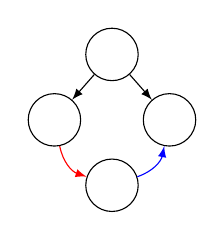
\begin{tikzpicture}[
            scale=1,
            transform shape,
            node distance=.35cm and .25cm,
            minimum width={width("Xtil")+2pt},
            minimum height={width("Xtil")+2pt},
            mynode/.style={draw,ellipse,align=center}
        ]
            \node[mynode] (Gi) {$\vG$};
            \node[mynode, below left=of Gi] (X) {$\vX$};
            \node[mynode, below right=of Gi] (Y) {$\vY$};
            \node[mynode, below right=of X] (C) {$\vC$};

            \path (Gi) edge[-latex] (X)
            (Gi) edge[-latex] (Y);
            % (X) edge[-latex] (C);
            \path [red, bend right](X) edge[-latex] (C);
            \path [blue,bend right](C) edge[-latex] (Y);
            % \path [red,bend right] (Gi) edge[-latex] (C);
        \end{tikzpicture} & \textit{(b)} & \rotatebox{90}{\hspace{0.65em} \scriptsize \textsc{Ground-truth} ($\vG$) } & 
        \includegraphics[width=0.3\textwidth]{figures/cf-mat-wo-rec} & \textit{(c)} &
        \includegraphics[width=0.3\textwidth]{figures/cf-mat-w-rec} 
    \end{tabular}

    \caption{
    %
    \textit{(a)} Graphical model of our setup:  the \textbf{black} arrows encode the data generation process, the \textcolor{red}{\textbf{red}} arrow indicate the learned concept distribution, and the \textcolor{blue}{\textbf{blue}} arrow the reasoning module.
    %
    \textit{(b)} Confusion matrices of (Boolean) concepts learned by DeepProblog for our three bits XOR task without any mitigation strategy, and
    %
    \textit{(c)} with a reconstruction term, cf. \cref{eq:solutions-reasoning-rec}.
    %
    In both cases the learned concepts are consistent with the knowledge and in the second one they also manage to reconstruct the input.  %Additionally, reconstruction allows to map distinct ground-truth concept vectors into distinct predicted concept vectors.
    The confusion matrices immediately show that, despite this, the learned concepts are reasoning shortcuts.
    }
    \label{fig:generative-process}
\end{figure}


We consider a NeSy prediction task where, given sub-symbolic inputs $\vX$, the goal is to infer one or more labels $\vY \in \{0, 1\}^\ell$ consistent with a given propositional formula $\BK$ encoding prior knowledge.
%
We focus on DeepProbLog~\citep{manhaeve2018deepproblog}, a representative and sound framework for such tasks.
%
From a probabilistic perspective, DeepProbLog:
%
(i) Extracts $k$ concepts $\vC \in \{0, 1\}^k$ from a $\vX$ via a neural network $p_\theta (\vC \mid \vX)$, and
%
(ii) Models the distribution over the labels $\vY$ as a uniform $u_\BK (\vy \mid \vc) = \Ind{(\vy, \vc) \models \BK}$.
%
The label distribution is obtained by marginalizing $\vC$:
%
\[
    \textstyle
    p_\theta(\vy \mid \vx; \BK) = \sum_\vc u_\BK(\vy \mid \vc) p_\theta(\vc \mid \vx)
    \label{eq:deepproblog}
\]
%
DeepProbLog is then trained via \textit{maximum likelihood}. \hspace{0.3em}
%
In order to understand when doing so recovers concepts $\vC$ with the ``correct semantics'', we have to first define the unobserved generative mechanism underlying the training data whose concepts we wish to identify.
%
Motivated by work on identifiability in (causal) representation learning \citep{locatello2019challenging, scholkopf2021toward, khemakhem2020variational, ahuja2022towards}, we assume there exist $k$ ground-truth concepts $\vG \in \{0, 1\}^k$ spanning a space $\calG$,
%\footnote{Notice that the support of $\vC$ corresponds to all concepts accounted in the knowledge $\BK$, so it coincides with $\calG$. \ST{unclear; is this necessary?}} 
and that the examples $(\vX, \vY) = (f( \vG ), h(\vG))$ are generated by an invertible function $f: \calG \to \mathcal X \subset \bbR^d$ and a surjective function $h: \calG \to \calY$, with $|\calY| \leq |\calG|$.
%
Here, $h$ plays the role of the ground-truth reasoning module that infers the label $\vY$ from the ground-truth concepts $\vG$ according to $\BK$, while $f$ generates the observations themselves.\footnote{Due to space constraints, we assume $\vX$ depends on $\vG$ only.  In practice, it might also depend on additional ``stylistic'' factors of variation (e.g., font)~\citep{von2021self}. Our results apply to this more complex case with minimal modifications.}
%
Cf. \cref{fig:generative-process} for an illustration.
%
In the next sections, we will show how maximum likelihood training can recover the mechanism $g \circ f^{-1}$, but not the ground-truth mapping from inputs to concepts $f^{-1}$, \ie the ``correct semantics''.

% Concerning the inference mechanism, we consider a factorized distribution $p_\theta (\vC, \vY \mid \vX; \BK) =  p_\theta(\vY \mid \vC; \BK)  p_\theta(\vC|\vX)$ with learnable parameters $\theta$. 
% %
% Here, the variables $\vC$ represent the learned concepts which are typically encoded via neural networks. Without loss of generality, the prediction of $\vY$ depends solely on the concepts $\vC$, since they contain all relevant information for the classification problem. 
% %
% For instance, DeepProblog \citep{manhaeve2018deepproblog} infers $\vY$ by grounding a probabilistic logic program based on the knowledge $\BK$ on the ...

% In the rest of the paper, we consider only the probability decomposition given by DeepProblog, and we leave a general characterization for future works.

\section{Reasoning shortcuts and mitigation strategies}

We consider training points $(\vx, \vy) \in \dataset_{\vX, \vY}$, each originated by corresponding ground-truth concepts $\vg \in \dataset_\vG$.\footnote{We assume the training examples are \textit{noiseless} and cover all possible combinations of ground-truth factors $\vG$, as even this ``ideal'' setting admits RSs.}  Our starting point is the log-likelihood, which constitutes the objective of training:
%
\[
    \textstyle
    \calL(\theta) := \sum_{ (\vx,\vy) \in \dataset_{\vX, \vY}} \log p_\theta(\vy \mid \vx; \BK) \equiv \sum_{ \vg \in \dataset_{\vG} } \log  p_\theta \big( h(\vg) \mid f(\vg); \BK  \big)
    \label{eq:log-lh-nesy}
\]
%
Notice that all optima of \cref{eq:log-lh-nesy} satisfy $p_\theta (\vy \mid \vx; \BK  ) = 1$ for all examples.  By \cref{eq:deepproblog}, this entails that any $\vc \sim p_\theta( \vc \mid \vx )$ must satisfy the knowledge $\BK$, that is, $(\vc, \vy) \models \BK$ (see \citep[Theorem 3.2]{marconato2023neuro}).
%
How many alternative distributions $p_\theta(\vc \mid \vg) := p_\theta(\vc \mid f(\vg))$ do attain maximum likelihood?  Since $p_\theta$ is a neural network, there may be infinitely many, yet all of them except one are RSs.  This is sufficient to show that \textit{RSs cannot be discriminated from the ground-truth concept distribution based on likelihood alone}~\citep{marconato2023neuro}.

Importantly, it turns out all optimal distributions $p_\theta(\vc \mid \vx)$ are convex combinations of the \textit{deterministic} optima (\textit{det-opts}), that is, those distributions $p_\theta(\vc \mid \vg)$ mapping each $\vg$ to a unique $\vc$ with probability one.
%
If the likelihood admits a single \textit{det-opt}, this is also the \textit{only} solution and -- by construction -- it recovers the ground-truth concepts.  \textit{RSs arise when there are two or more det-opts}.
%
How many det-ops are there?  Let $S_\vy = \big \{ \vc \, : \, (\vc, \vy) \models \BK \big \}$ be the set of $\vc$'s that $\BK$ assigns to label $\vy$.
%
Notice that if $p_\theta(\vc \mid \vg)$ attains maximum likelihood, then any $\vc \sim p_\theta(\vc \mid \vg)$ falls within $S_{h(\vg)}$.
%
In this sense, a \textit{det-opt} implicitly maps each vector $\vg \in \calG$ to a vector $\vc \in S_{h(\vg)}$.
%
This gives us a mechanism to count \textit{det-opts}: for each $\vg$ there are exactly $|S_{h(\vg)}|$ vectors $\vc$ that it can be mapped to, meaning that number of \textit{det-opts} for \cref{eq:log-lh-nesy} is:
%
\begin{equation}
    \textstyle
    \#\text{det-opts}(\calL) = \prod_{\vy \in \calY} |S_\vy |^{|S_\vy|}
    \label{eq:solutions-to-reasoning}
\end{equation}
%
As a consequence, the ground-truth concepts can only be retrieved if $|S_\vy| = 1$, \ie each label $\vy$ can be deduced from a unique $\vc$.
%(and, consequently, $|\calY| = |\calG|$).
%
This is seldom the case in NeSy tasks, meaning that maximizing the likelihood of the labels $\vY$ cannot rule out RSs in general.

In the following, we discuss two natural mitigation strategies and their impact in reducing the total number of \textit{det-ops}.

\paragraph{Reconstruction is insufficient.}  Given the likelihood is incapable of discriminating intended and RS solutions, one option is to augment it with a term encouraging learned concepts $\vC$ to capture information necessary to reconstruct the input $\vX$, for instance:
%
\[
    \textstyle
    \calR (\theta) := \sum_{\vx \in \dataset_\vX} \big[ \sum_{\vc} p_\theta (\vc \mid  \vx) \log p_\psi( \vx \mid \vc ) \big] \equiv \sum_{\vg \in \dataset_\vG} \big[ \sum_{\vc} p_\theta (\vc \mid  \vg) \log p_\psi( \vg \mid \vc )  \big]
    \label{eq:rec-term}
\]
%
Here, $p_\psi(\vx \mid \vc)$ is the distribution output by a neural decoder with parameters $\psi$, and we introduced $p_\psi (\vg \mid \vc) := p_\psi(f(\vg) \mid \vc)$. 
%
The optima of \cref{eq:rec-term} must satisfy $p_\psi(\vg \mid \vc) = 1$ for all $\vc \sim p_\theta(\vc \mid \vg)$.
%
In other words, restricting again to \textit{det-ops} for the encoder, the only \textit{det-ops} that ensure perfect reconstruction are those mapping distinct $\vg$'s to distinct $\vc$'s, \ie that ensure the encoder is injective.
%
How many such \textit{det-opts} are there?  Notice that these \textit{det-opts} can be enumerated by taking each $\vg \in \calG$ in turn and mapping it to an arbitrary $\vc$ in $S_{h(\vg)}$ \textit{without replacement} (to ensure injectivity), until all $\vg$'s have been mapped.
%
%When combining the two objectives in \cref{eq:log-lh-nesy} and \cref{eq:rec-term}, a \textit{det-opt} implicitly defines a permutation on the elements of $S_{\vy}$, so that the number of possible solutions amounts to $|S_\vy |!$ for each $\vy$.
%
This entails that the number of \textit{det-opt}s -- under perfect reconstruction -- becomes:
%
\[
    \textstyle
    \#\text{det-opts}(\calL + \calR) = \prod_{\vy \in \calY} |S_\vy| !
    \label{eq:solutions-reasoning-rec}
\]
%
% Notice that, in this case, convex combinations of \textit{det-opts} are no longer valid solution as they would not optimize the reconstruction term.
Once again, unless $|S_\vy|=1$ for all $\vy$'s, there are multiple possible solutions, most of which are RSs.
% Nonetheless, the scaling of the possible solutions remains factorial with the dimension of the equivalence classes, so
In other words, \textit{adding a reconstruction term can be insufficient to completely rule out learning reasoning shortcuts}.


\paragraph{The effect of concept supervision.}  Next, we consider a scenario where \textit{concept supervision} is provided (for all concepts) for at least some examples $(\vx, \vg) \in \overline{\dataset}_{\vX, \vG}$.  We consider the $L_2$ loss for fitting the supervision, for simplicity:
%
\[
    \textstyle
    \calC (\theta) \propto  \sum_{(\vx, \vg) \in \overline{\dataset}_{\vX, \vG} }  ( \vc - \vg)^2 p_\theta (\vc \mid \vx)  \equiv \sum_{\vg \in \overline{\dataset}_{\vG}  }\sum_{\vc} ( \vc - \vg)^2 p_\theta (\vc \mid \vg) 
    \label{eq:concept-supervision-loss}
\]
%
The only concept distributions $p_\theta(\vc \mid \vg)$ minimizing \cref{eq:concept-supervision-loss} are those that allocate all probability mass to the annotated concepts.
%
Now, let $\nu_\vy$ be the number of vectors $\vc \in S_\vy$ for which we have supervision $\vg$, for a total of $|\overline{\dataset}_{\vG}| = \sum_\vy \nu_\vy$.
%
The situation is analogous to \cref{eq:solutions-to-reasoning} and \cref{eq:solutions-reasoning-rec}, except that now for exactly $\nu_\vy$ vectors $\vc$ we know exactly what $\vg$ they should be mapped to, leaving the remaining $|S_\vy| - \nu_\vy$ vectors dangling.  This gives:
% Upon optimizing \cref{eq:concept-supervision-loss} we disambiguate the concepts in $\overline{\dataset}_\vG$, Hence, the number of total \textit{det-opt}s becomes:
%
\[
    \textstyle
     \# \text{det-opts}(\calL + \calC)  = \prod_{\vy \in \calY} |S_\vy|^{ |S_\vy| - \nu_\vy  }, \quad \quad \# \text{det-opts}( \calL + \calR + \calC)  = \prod_{\vy \in \calY} ( |S_\vy| - \nu_\vy )!
     \label{eq:total-sol-concepts}
\]
%
Here, the first term counts how many \textit{det-opt}s optimize both the label likelihood and the concept supervision, and the second one those optimizing the likelihood, reconstruction and concept supervision.
%
This shows providing concept supervision can dramatically reduce the number of \textit{det-opts} but also that \textit{a substantial amount is necessary to rule out all RSs}. \newpage
%
% When combining all terms, the number of total concepts that need to be supervised to identify the ground-truth mechanism $f^{-1}$ amounts to: $ \nu = \sum_{\vy \in \calY} (|S_\vy| -1) = |\calG \mid - |\calY| $.


\section{Empirical Verification}

We outline a toy experiment showing how reasoning shortcuts affect even a simple NeSy task. 
%
Let $\vg = (g_1, g_2, g_3)$ be three bits and consider the task of predicting their parity, that is, $y = g_1 \oplus g_2 \oplus g_3$.
%
Each label $y \in \{0, 1\}$ can be deduced from $4$ possible concept vectors $\vg$.
%
We train two MLPs, one encoding directly $\vg$ into $p_\theta (\vc \mid \vg)$, and another decoding $\vc$ into $p_\psi(\vg \mid \vc)$.  Labels are predicted as per \cref{eq:deepproblog}.
%
Given the problem at hand, the total number of \textit{det-opt}s is given by \cref{eq:solutions-to-reasoning} and by \cref{eq:solutions-reasoning-rec}:
%
$$ \# \text{det-opts}(\calL) = (4^4 \cdot 4^4) \quad \quad
\# \text{det-opts}(\calL + \calR) = (4! \cdot 4!)
$$
%
Empirically, what happens is that without concept supervision, the model picks up reasoning shortcuts to solve the task.
%
\cref{fig:generative-process} shows two such RSs, both optimal, obtained by our model when optimizing \textit{(b)} only the likelihood, and \textit{(c)} both the likelihood and the reconstruction term.  In both cases, the solutions fail to recover the ground-truth concepts.

\section*{Conclusion.} Our results altogether show that the ground-truth concepts are hard, if not impossible, to recover empirically, and that two natural mitigation strategies do not completely address the problem.
%
In particular, the amount of concept supervision required grows linearly with the number of possible concept combinations.
%
We envisage well-tuned strategies based on targeted concept-supervision, combined with additional restrictions on the model itself (and specifically \textit{disentanglement} between concepts~\citep{suter2019robustly}), will likely facilitate (provable) identification of the ground-truth concepts.
%
This is left to future work.

\section*{Acknowledgements}

The research of ST and AP was partially supported by TAILOR, a project funded by EU Horizon 2020 research and innovation programme under GA No 952215.


%%
%% Define the bibliography file to be used
\bibliographystyle{unsrtnat}
\bibliography{references.bib}

%%
%% If your work has an appendix, this is the place to put it.

\end{document}